\section{Descrizione apparato sperimentale}	
\label{sec:DEscrizioneApparatoSperimentale}

	Il sistema di controllo fornito in laboratorio si basa sul programma \textit{Real-Time Workshop} che permette l'esecuzione in tempo reale di controllori implementati tramite \textit{Matlab-Simulink}. L'apparato sperimentale è rappresentato in figura \ref{fig:apparatoSperimentale}.
	
	\begin{figure}[H]
		\centering
		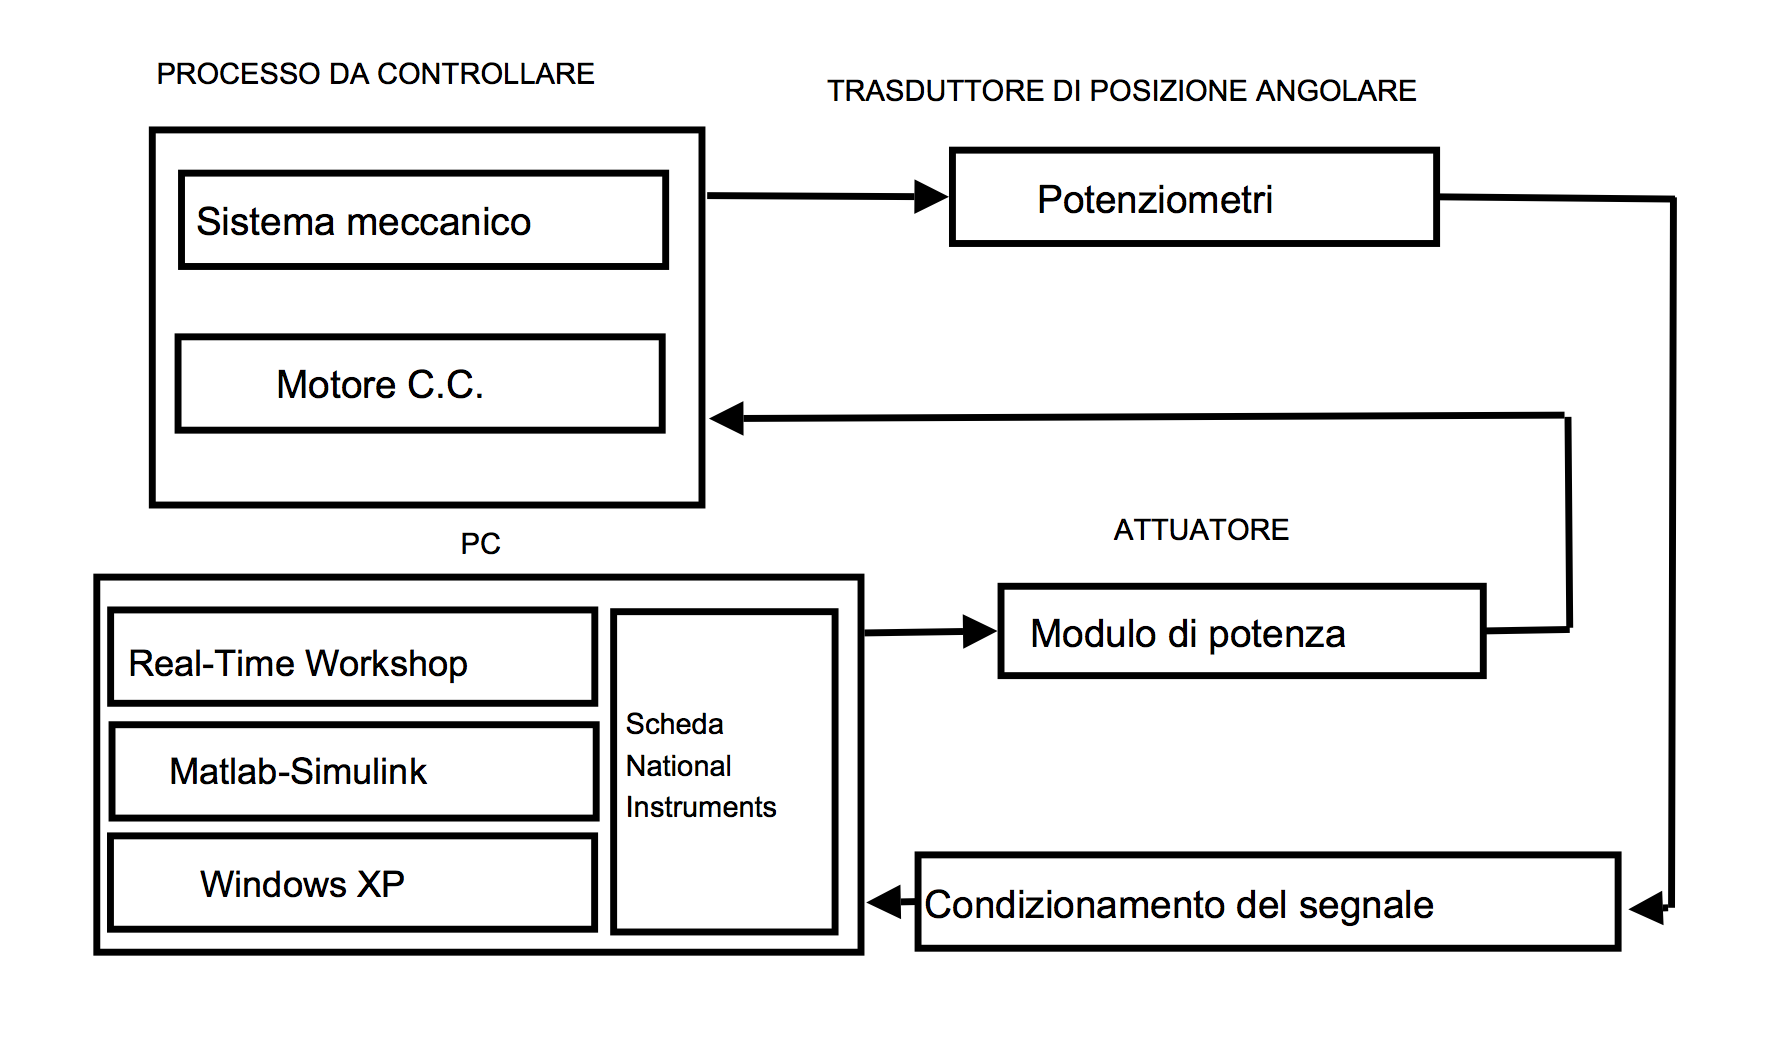
\includegraphics[width=1\textwidth]{./figure/apparato_sperimentale}
		\caption{Schema componenti dell'apparato sperimentale.}
		\label{fig:apparatoSperimentale}
	\end{figure}
	
	\begin{figure}[H]
		\centering
		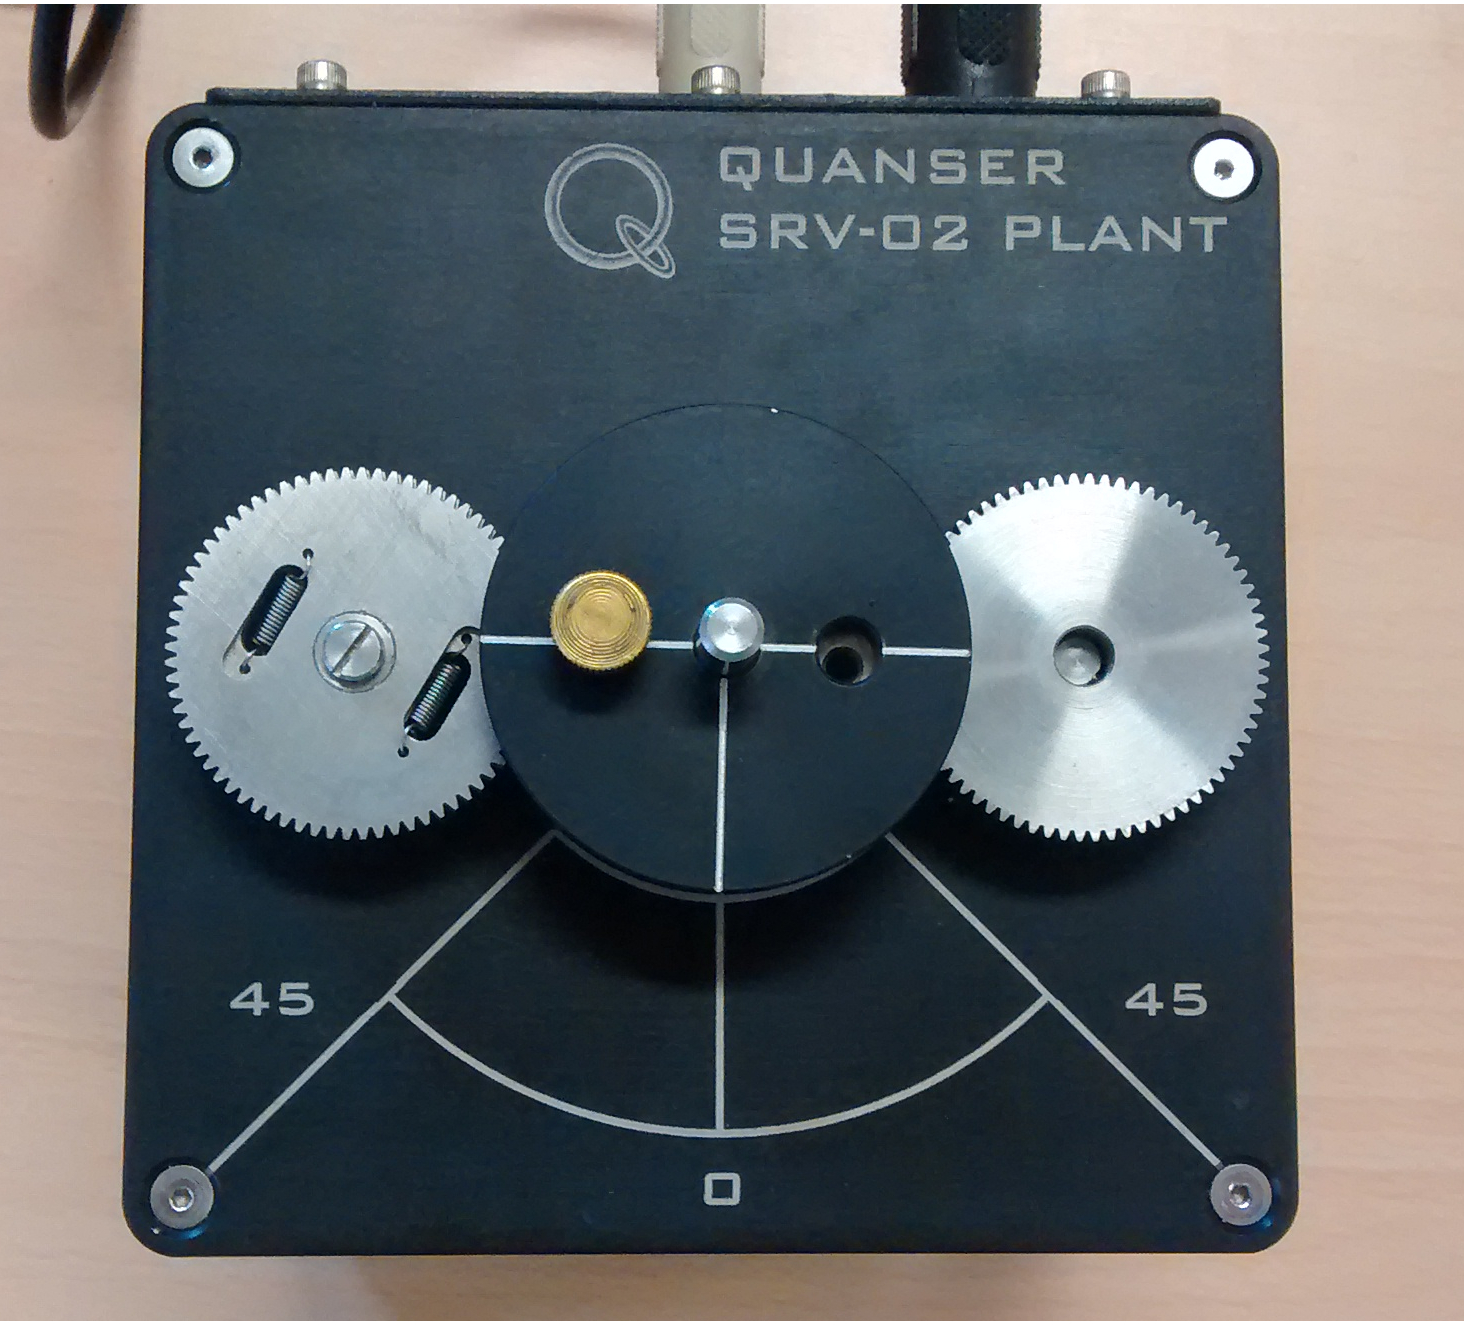
\includegraphics[width=0.45\textwidth]{./figure/motore}
		\caption{Sistema elettromeccanico da controllare (vista dall'alto)}
		\label{fig:fotoMotore}
	\end{figure}
	
	\begin{figure}[!ht]
		\centering
		\subfloat[Modulo di potenza]
		{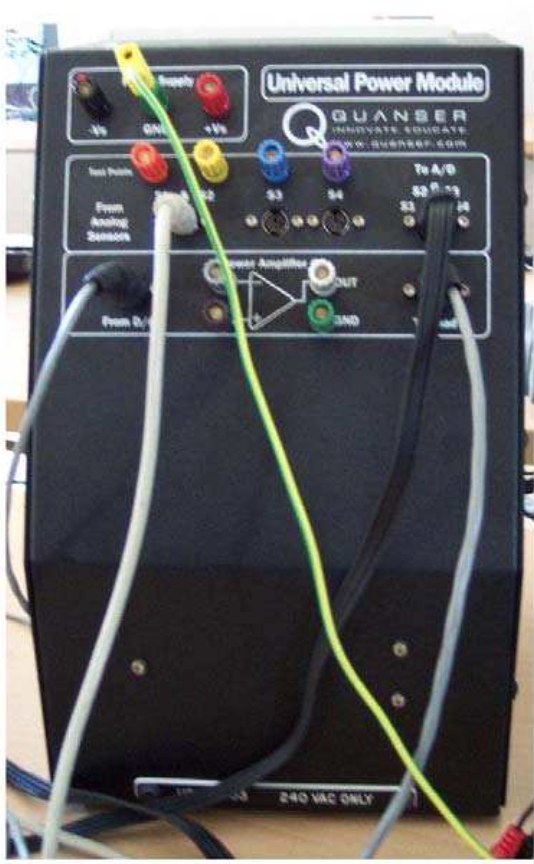
\includegraphics[width=0.3\textwidth,height=0.45\textwidth]{./figure/alimentatore}
		\label{fig:fotoModuloPotenza}}
		\subfloat[Scheda di acquisizione PCI]
		{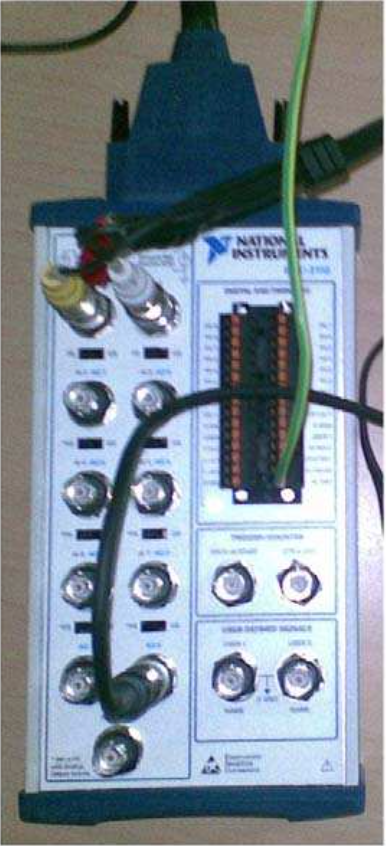
\includegraphics[width=0.3\textwidth,height=0.5\textwidth]{./figure/PCI}
		\label{fig:fotoSchedaNational}}
		\caption{Componenti dell'apparato sperimentale}
	\end{figure}
	
	\noindent Il processo da controllare è costituito da un sistema elettromeccanico comandato da un motore in corrente continua con motoriduttore. Quest'ultimo muove altre due ruote dentate, quella centrale che rappresenta il carico e ha lo scopo di indicare la posizione e il movimento in gradi della ruota, mentre nella seconda ruota (quella più esterna) è montato un trasduttore (costituito da un potenziometro) che converte la posizione in gradi del carico in segnale elettrico. Da notare che il sistema a tre ruote serve per ridurre l'effetto di \textit{backlash} al carico ovvero il gioco che esiste fra due ingranaggi qualunque per il semplice fatto che le tolleranze meccaniche non permettono di avere un accoppiamento perfetto. A causa di questo fenomeno si ha un ritardo nell'inversione del moto su un asse rispetto al comando stesso di inversione. Per comandare tutto ciò si è utilizzato un modulo di potenza costituito da un alimentatore DC duale da 12V e da un amplificatore lineare che è in grado di fornire al motore $\pm 5$V. L'acquisizione dati è stata fatta con la scheda \textit{National Instruments PCI-6221} accessibile via software attraverso porte I/O. In figura \ref{fig:fotoMotore} si osservano i diversi componenti che costituiscono il sistema elettromeccanico da controllare e in figura \ref{fig:fotoModuloPotenza} si nota il modulo di potenza utilizzato assieme alla scheda di acquisizione dati in figura \ref{fig:fotoSchedaNational}. In figura \ref{fig:blocchiSimulink} sono raffigurati blocchi che permettono la comunicazione tra Matlab-Simulink e la scheda PCI che a sua volta, tramite il modulo di potenza, è connessa al motore e al trasduttore.
	
	\begin{figure}[!h]
		\centering
		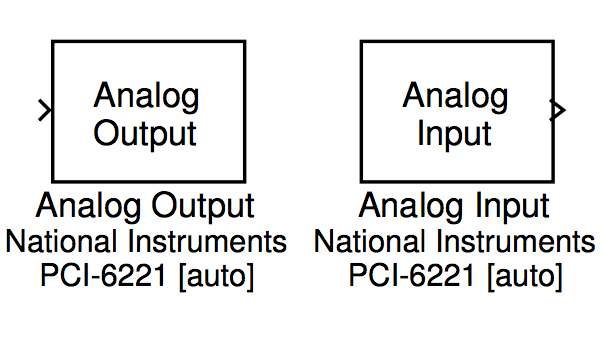
\includegraphics[width=0.3\textwidth]{./figure/blocchi_simulink}
		\caption{Blocchi Simulink per la prova sperimentale}
		\label{fig:blocchiSimulink}
	\end{figure}